\documentclass{article}
\usepackage{tikz}
\usetikzlibrary{positioning}

\begin{document}

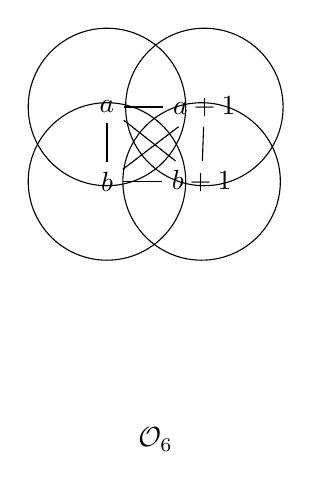
\begin{tikzpicture}[node distance=0.5cm]
    \node (a) {$a$};
    \node[right=of a] (b) {$a+1$};
    \node[below=of a] (c) {$b$};
    \node[right=of c] (d) {$b+1$};

    \draw (a) -- (b);
    \draw (a) -- (c);
    \draw (a) -- (d);
    \draw (b) -- (c);
    \draw (b) -- (d);
    \draw (c) -- (d);

    \draw[dotted] (a) -- (d);
    \draw[dotted] (b) -- (c);

    \draw (a) circle (1);
    \draw (b) circle (1);
    \draw (c) circle (1);
    \draw (d) circle (1);

    \node[below=2cm] at (current bounding box.south) {$\mathcal{O}_6$};
\end{tikzpicture}

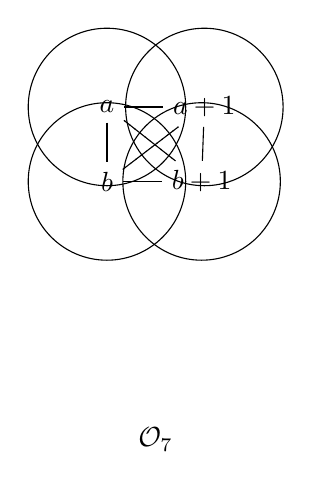
\begin{tikzpicture}[node distance=0.5cm]
    \node (a) {$a$};
    \node[right=of a] (b) {$a+1$};
    \node[below=of a] (c) {$b$};
    \node[right=of c] (d) {$b+1$};

    \draw (a) -- (b);
    \draw (a) -- (c);
    \draw (a) -- (d);
    \draw (b) -- (c);
    \draw (b) -- (d);
    \draw (c) -- (d);

    \draw[dotted] (a) -- (d);
    \draw[dotted] (b) -- (c);

    \draw (a) circle (1);
    \draw (b) circle (1);
    \draw (c) circle (1);
    \draw (d) circle (1);

    \node[below=2cm] at (current bounding box.south) {$\mathcal{O}_7$};
\end{tikzpicture}

\end{document}